\section{Dataset Analysis}
\label{sec:dataset}

To get a better understanding of the data and how it can be used we conducted a statistical analysis. Especially the distribution of errors within the dataset is important to understand the balance of the dataset and to understand the possible outcomes of our proposed models for error detection in human pose estimation.

\subsection{Distribution of Errors}

An important aspect of the dataset is the structure and distribution of data and their labels. In total, all 13 exercises mentioned in Section \ref{sec:exercises} were recorded twice. Each recording session consists of exactly 300 frames, resulting in a total of 7800 frames. Of these, every 10th frame was labelled for a total of 780 labelled frames, which were used for the preliminary model development.

When multiple persons are detected one person might be incorrectly detected in the background. While analysing the data the person that is not labelled as faulty is selected whenever possible. If a person is labelled as faulty, each joint is marked as in an unrealistic position.

An important factor in how well a model for HPE error detection can be trained on data is the balance of the dataset. In this case, the dataset is balanced by the error labels. 

\subsubsection{Full Body Error Distribution}

In Figure \ref{fig:fb_pie} the error distribution of the Full body problem set can be seen. It can be observed that the dataset is not very balanced.

\begin{figure}[ht]
  \centering
  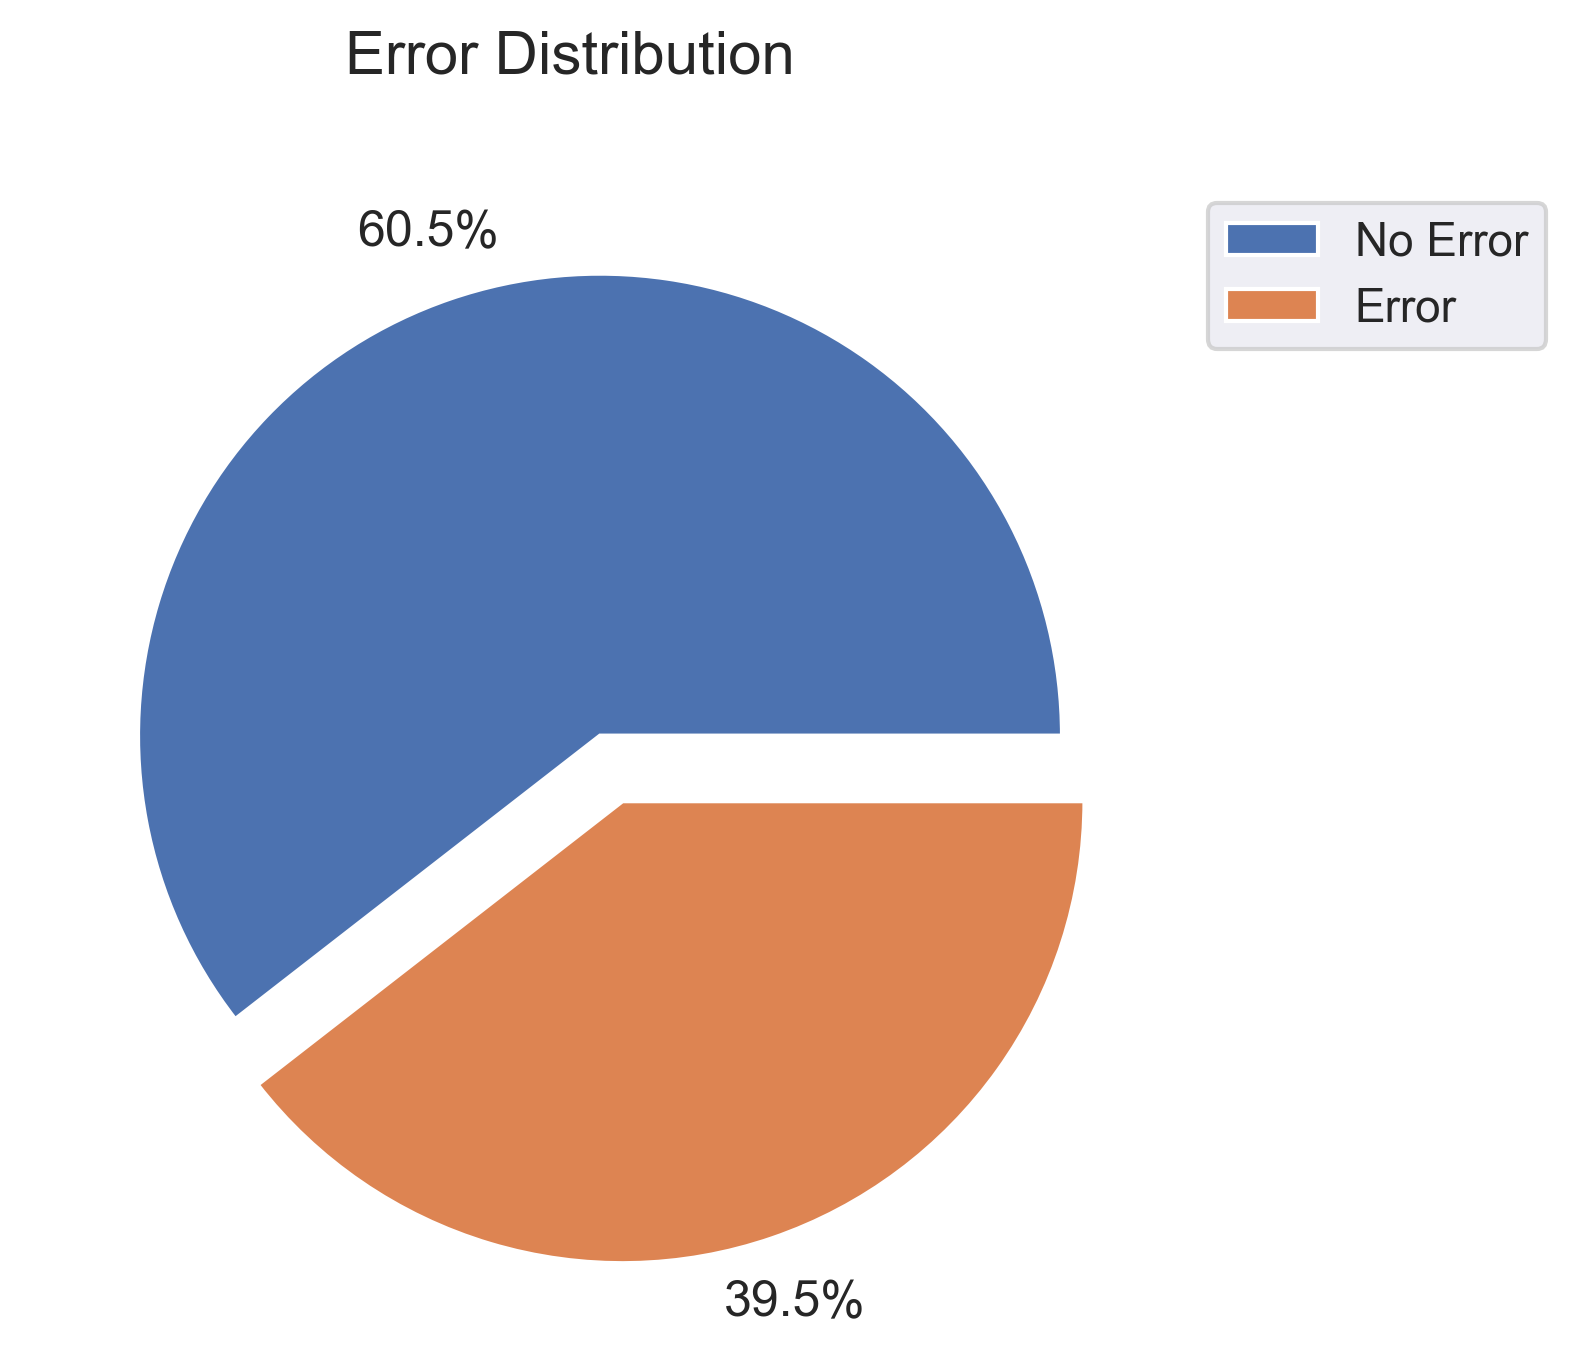
\includegraphics[width=0.5\textwidth]{figures/Data/dist_full_body/Error_Distribution.png}
  \caption[Error Distribution of the Full Body]{The distribution of Errors of the Full Body problem set. Of the 780 labelled frames, 308 are erroneous.}
  \label{fig:fb_pie}
\end{figure}

\subsubsection{Half Body Error Distribution}

Figure \ref{fig:hb_pie} shows a discrepancy between the error distribution of the lower body ($65.4\%$ Errors) and the upper body ($32.4\%$ Errors). The upper body is generally more stable and less error-prone than the lower body.

\begin{figure}[ht]
  \centering
  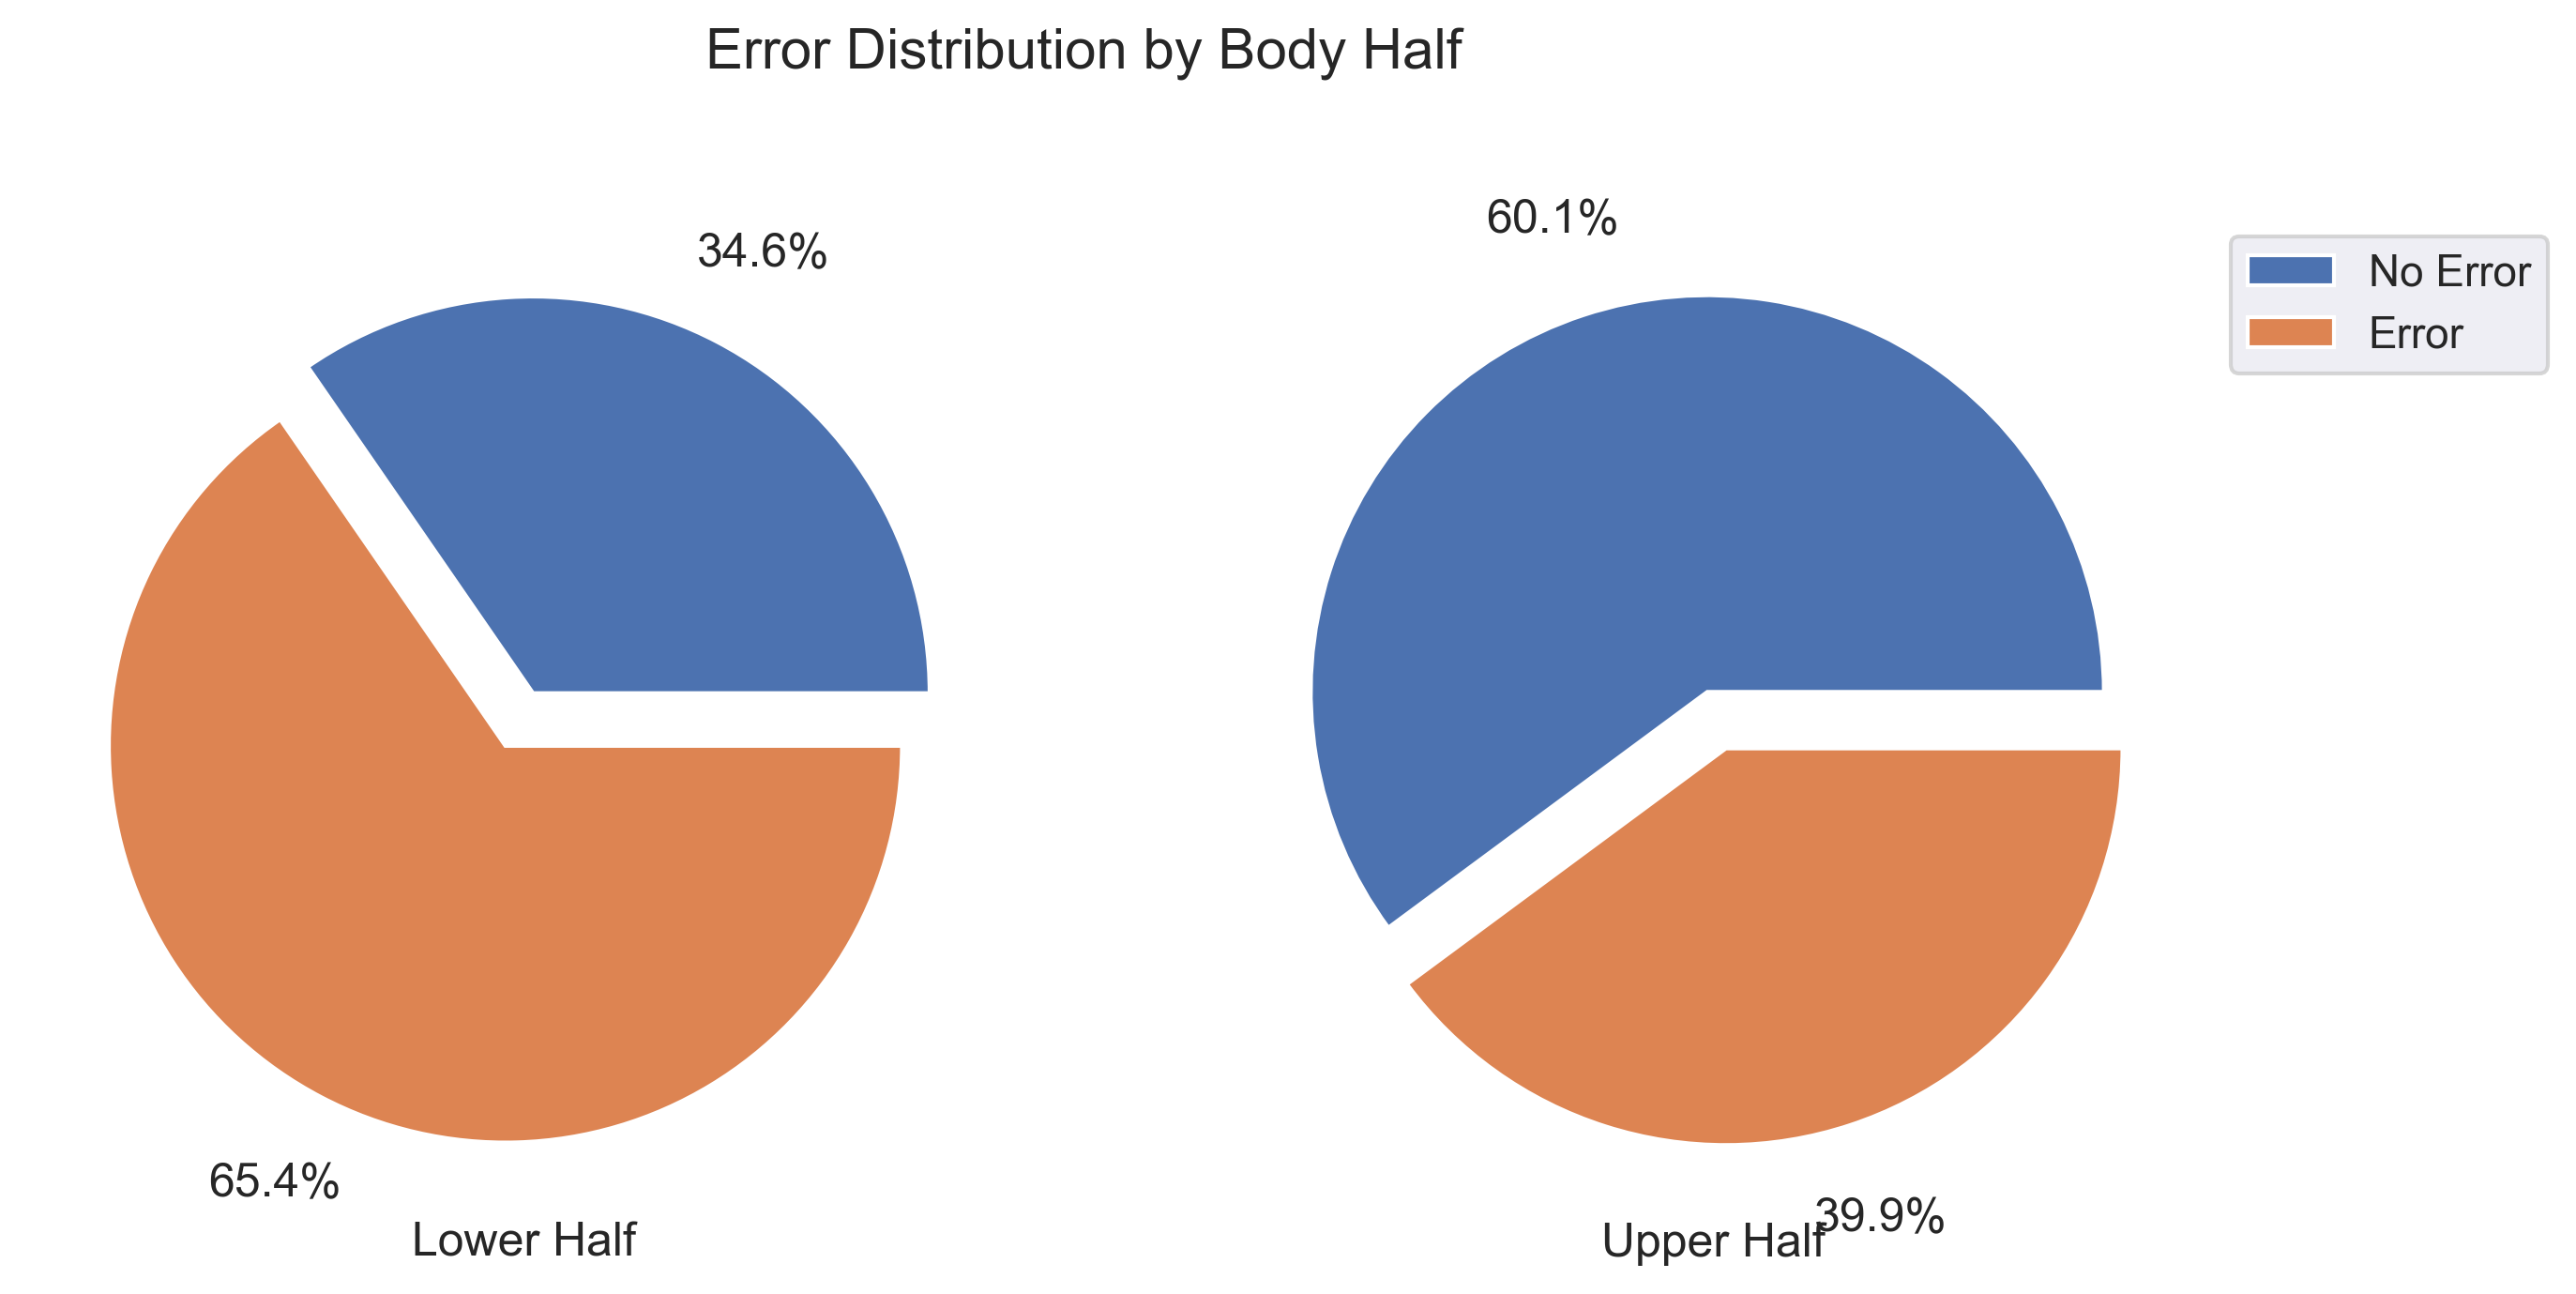
\includegraphics[width=0.7\textwidth]{figures/Data/dist_half_body/Error_Distribution_by_Body_Half.png}
  \caption[Error Distribution by Body Half]{The distribution of Errors of the Half Body problem set. Of the 780 labelled frames, 511 and 311 are erroneous for the lower and upper body respectively.}
  \label{fig:hb_pie}
\end{figure}

\subsubsection{Body part Error Distribution}

The error distribution of each body part is shown in Figure \ref{fig:lb_pie}. It can be observed that the errors of the body parts individually are very unbalanced. The left arm is the most error-prone body part with $24.1\%$ of the joints being faulty. The torso is the least error-prone body part with $10.3\%$ of the joints being faulty.

\begin{figure}[ht]
  \centering
  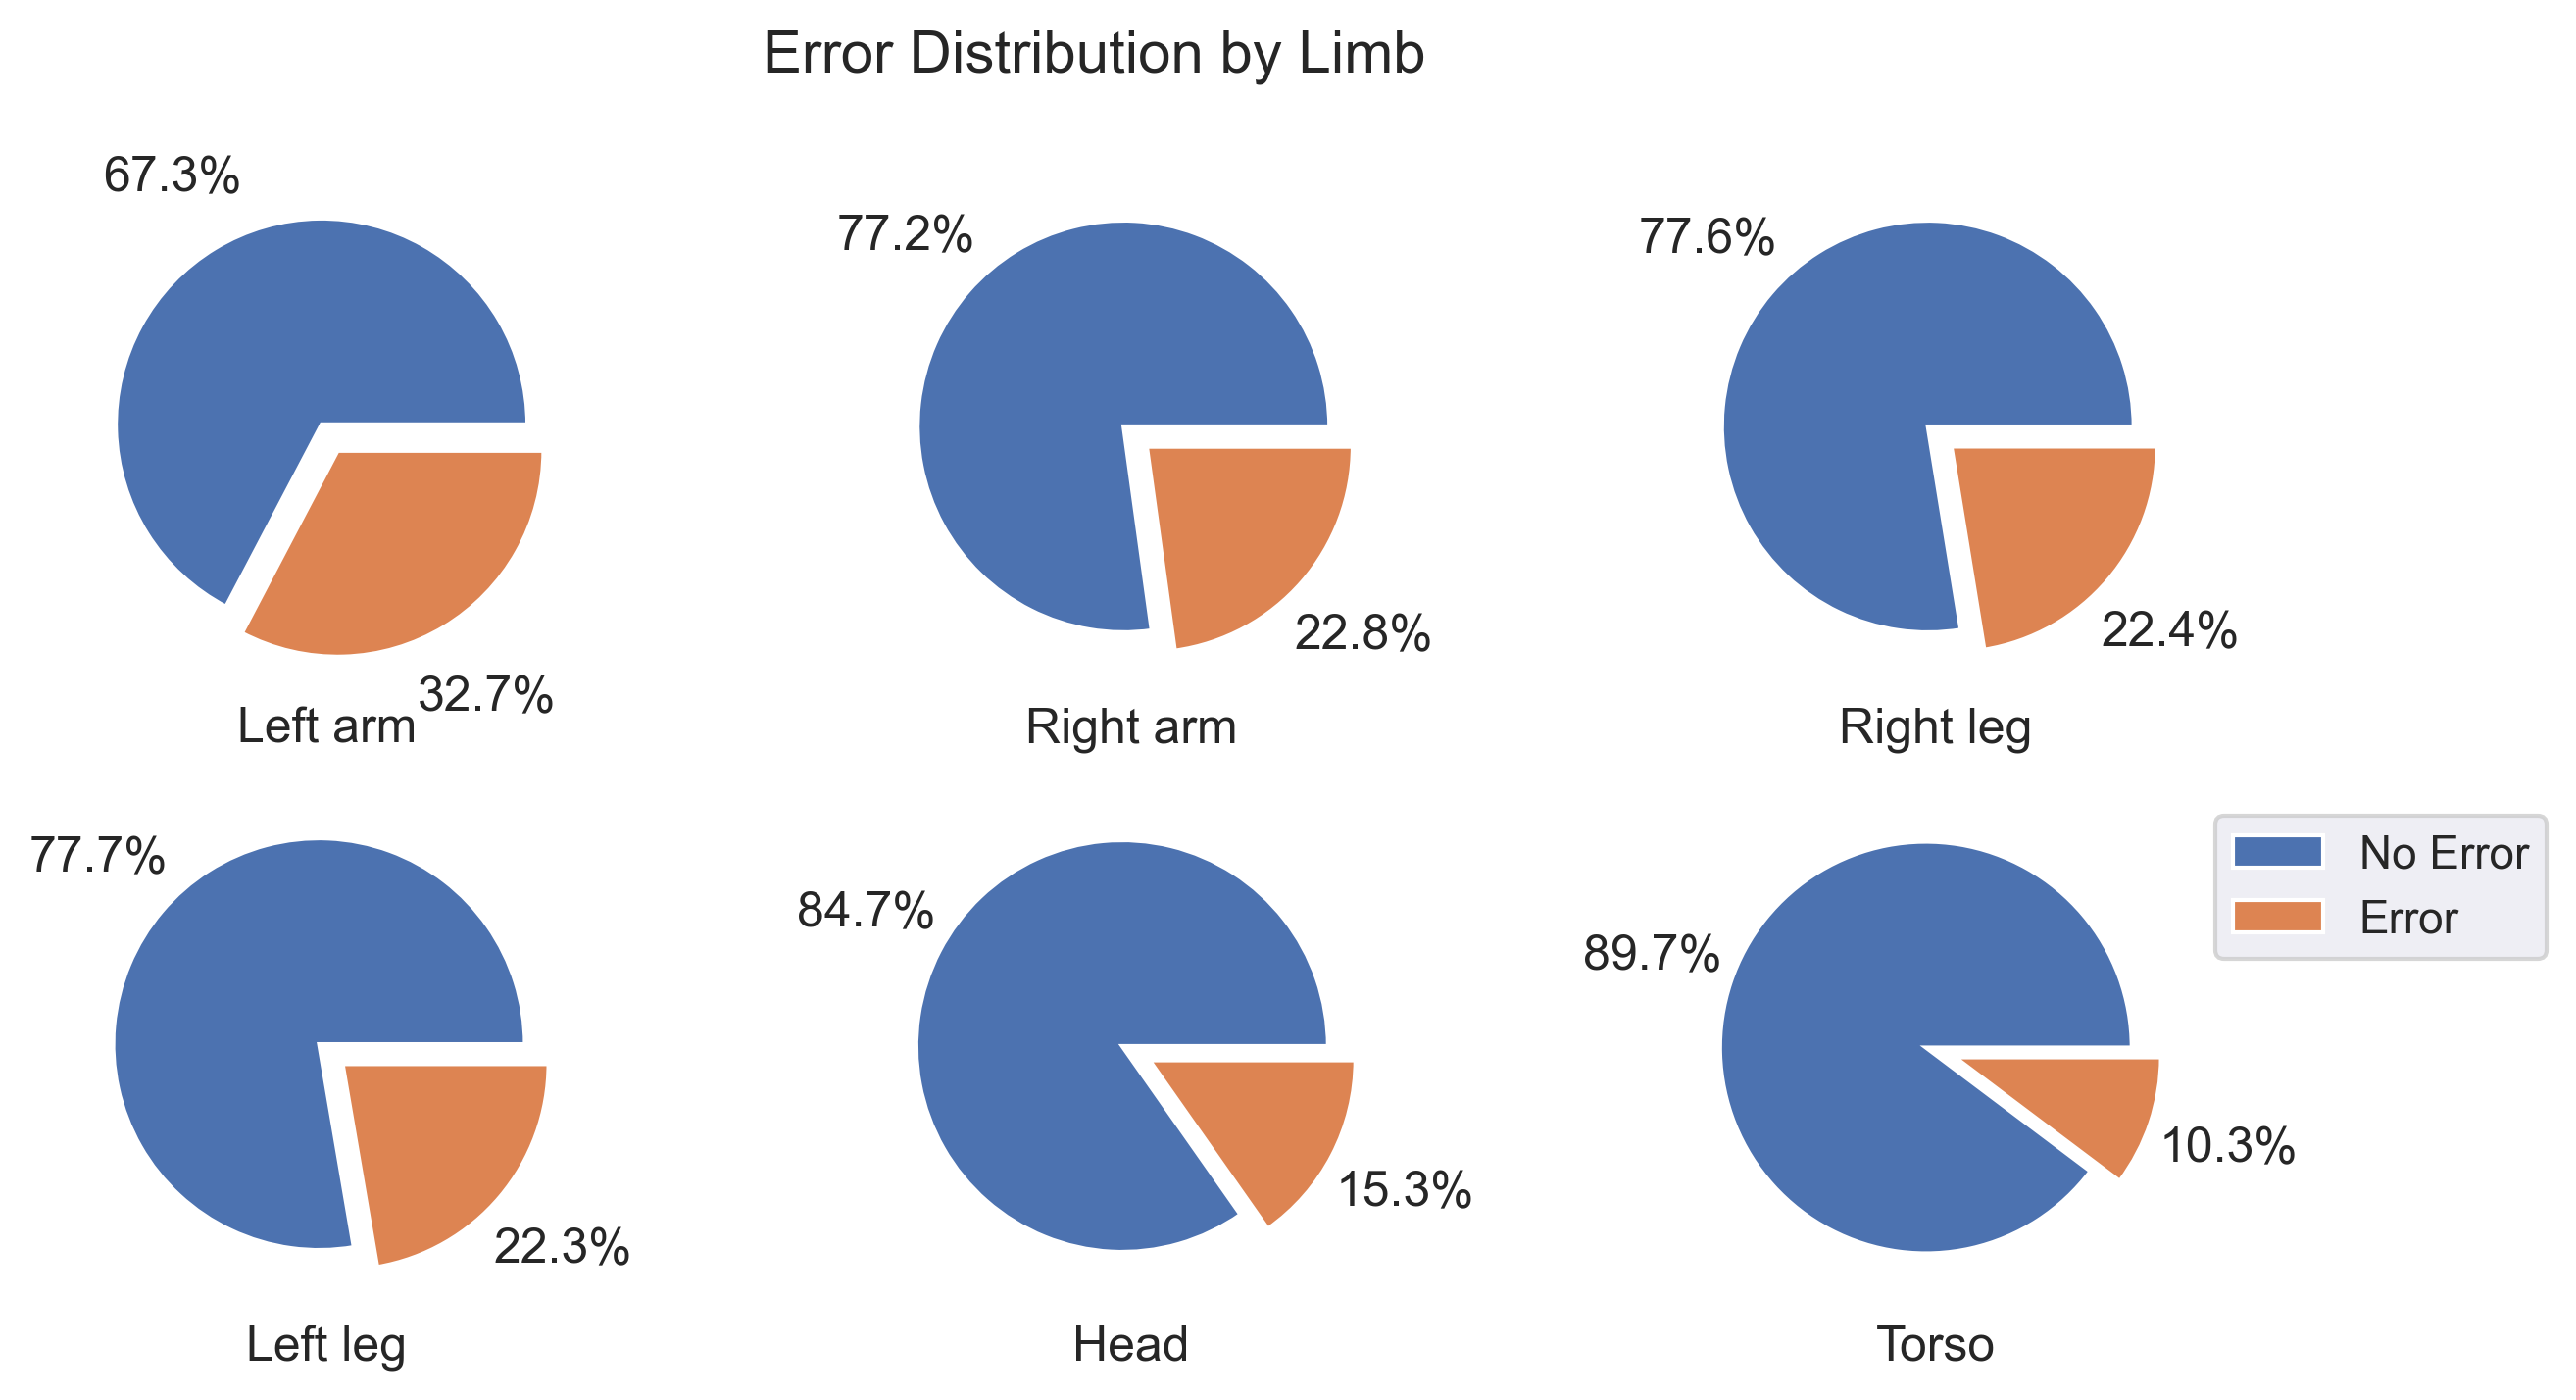
\includegraphics[width=0.8\textwidth]{figures/Data/dist_limbs/Error_Distribution_by_Limb.png}
  \caption[Error Distribution by Body part]{The distribution of errors of the Body Part problem set. The Left Arm is the most erroneous body part (255 errors), followed by the right arm (178 errors), the right leg (176 errors), the left leg (174 errors), and the head (119 errors). The least errors occur in the torso (80 errors in 780 frames).}
  \label{fig:lb_pie}
\end{figure}

\subsubsection{Joint Error Distribution}

Figure \ref{fig:jt_pie} shows that the major part of the errors that occur are errors with Label 2, i.e. the joint is detected at the wrong place. The second most common error is Label 1, i.e. the joint is not detected at all. The least common error is Label 3, i.e. the joint is detected in the approximate position of where another joint should be.

\begin{figure}[ht]
  \centering
  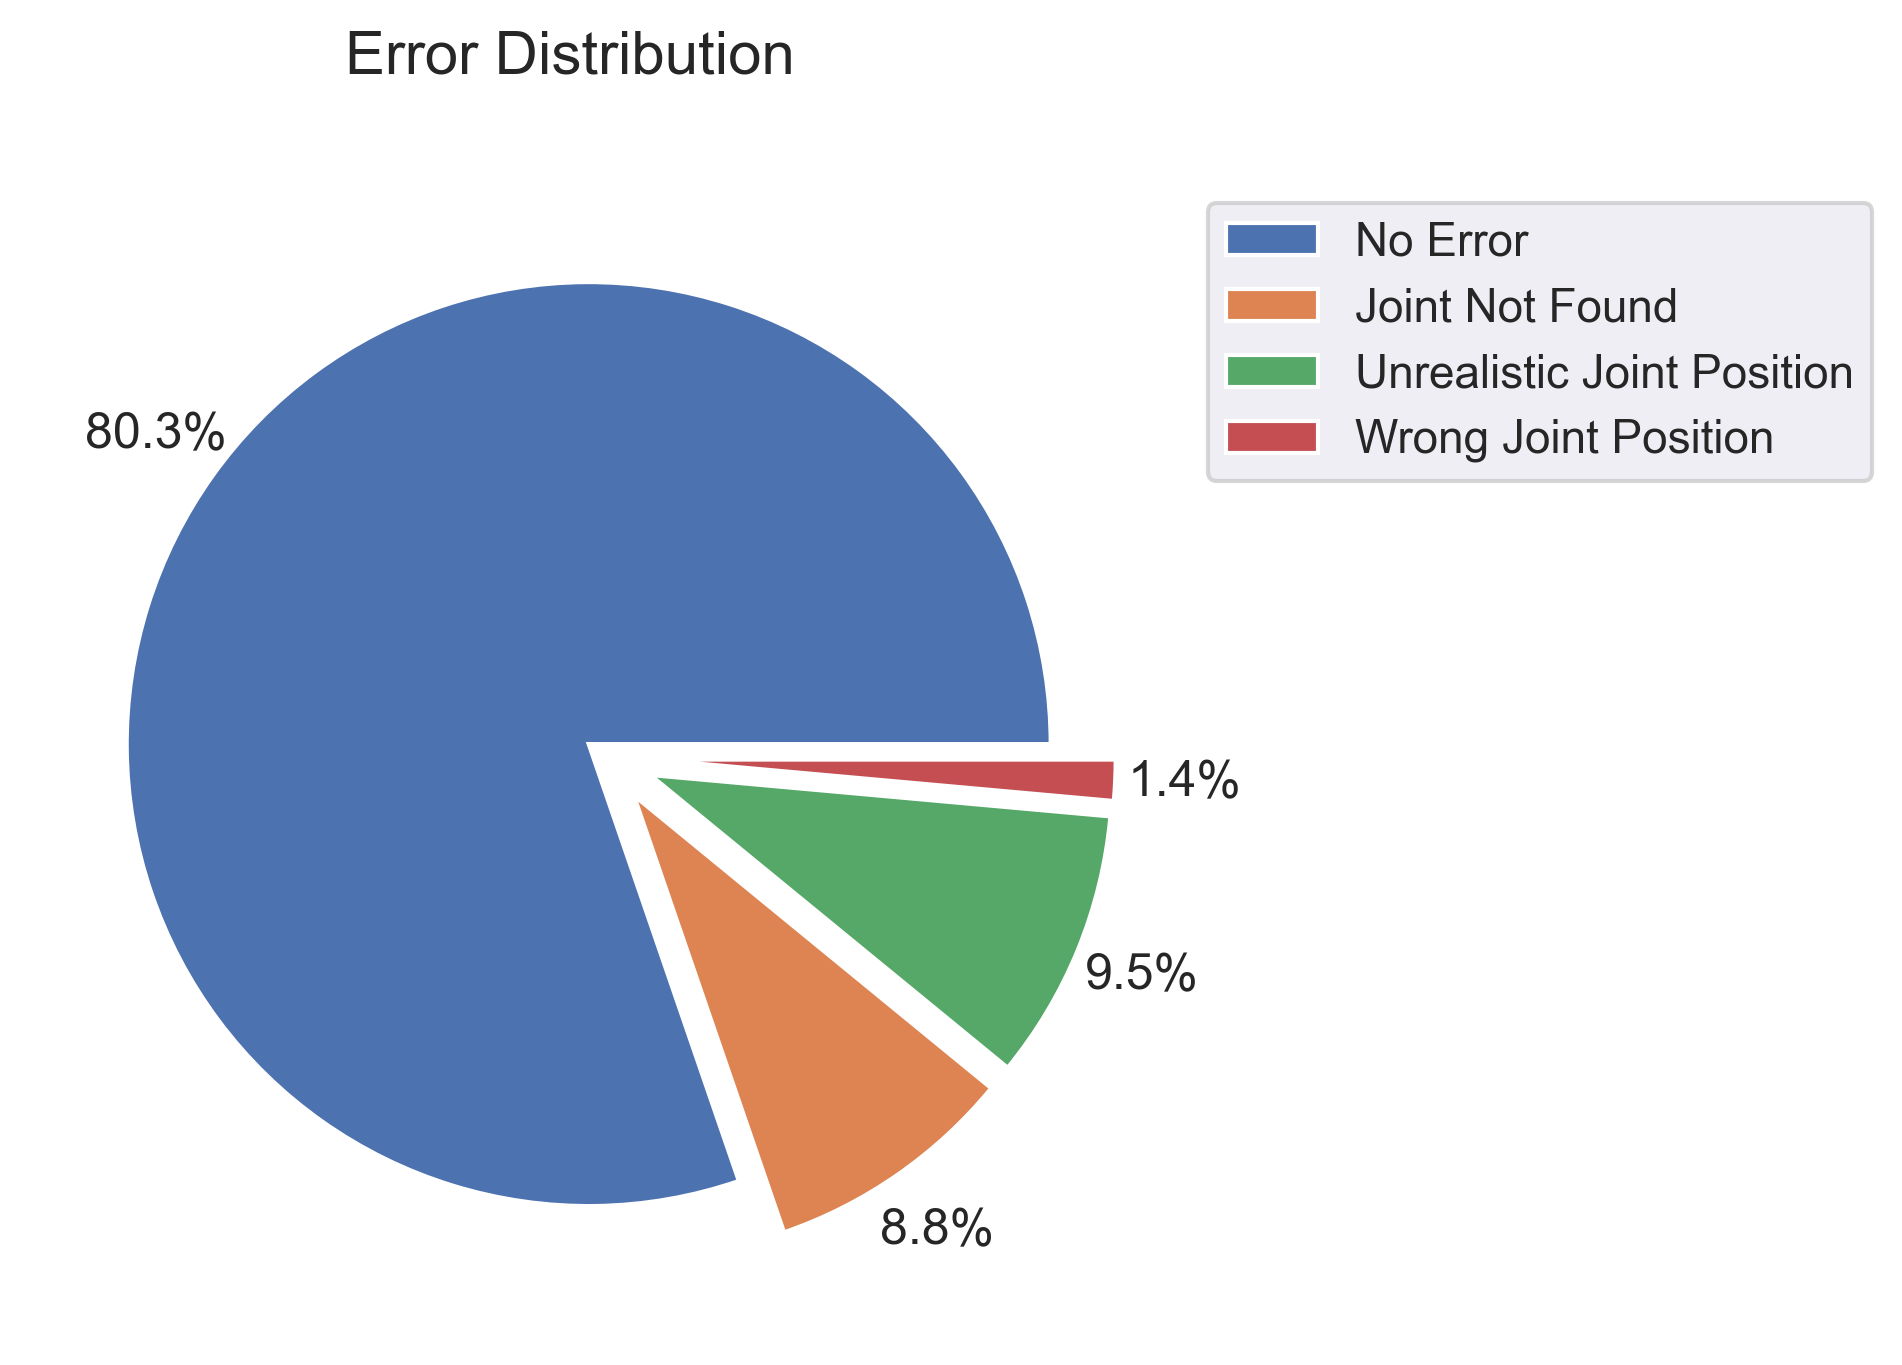
\includegraphics[width=0.5\textwidth]{figures/Data/dist_joints/Error_Distribution.png}
  \caption[Error Distribution for each error class]{The distribution of each error class. The Right Ankle is the most erroneous joint (542 errors), followed by the left ankle (520 errors), the left hand (249 errors), the left wrist (183 errors), the right hand (169 errors), the right wrist (146 errors), the left hip (136 errors), the right hip (122 errors), the right knee (147 errors), the waist (117 errors), the left knee (127 errors), the right elbow (101 errors), the left elbow (77 errors), the head (75 errors), the neck (73 errors), the right shoulder (65 errors), the right collar (63 errors), the torso (63 errors), and the left collar (63 errors). The least errors occur in the left shoulder (38 errors in 780 frames).}
  \label{fig:jt_pie}
\end{figure}

